\section{Existing Pipelines}

To generate a baseline to assess new methods against, Tesseract \cite{SmithTesseract}, a popular OCR engine sponsored by Google \cite{Vincent} and Ocular, another OCR engine based on Stochastic models were integrated into the pipeline using pytesseract \cite{Lee} and by calling jar files from python respectively.

\subsection{Tesseract}
\todo{TODO: ADD CONTENT}

\subsection{Ocular}
\todo{TODO: ADD CONTENT}

\section{Binarization}

\subsection{Evaluation Metrics}
\todo{NEW}

As there was no ground-truth information provided to compare binarizations against, visual comparison was utilized to determine which binarization method was providing the highest quality binarizations. This was done on four different images, which contained various features that would allow for quick visual evidence of the effectiveness of the methods \seefig{binarizationRaw}. The four images are of assorted sizes, from different collections, and are degraded to different degrees, allowing them to function as a valuable quick assessment tool without introducing bias into the evaluation of the methods.

To assess each binarization method, these images were used to determine how much of the ink on the papyrus was being included, and if noise was being added to the image in the form of background pixels being black or ink pixels being white. This metric was designed to ensure that the signal-to-noise ratio would be low and that the recall and precision would be high, even if they were not directly measurable without a ground truth for each pixel.

\begin{figure}
    \caption{Four Images Utilized to Visually Assess Binarization Quality}
    \label{fig:binarizationRaw}
    \begin{center}
        \begin{subfigure}[b]{0.45\textwidth}
            \centering
            \caption{Example File A}
            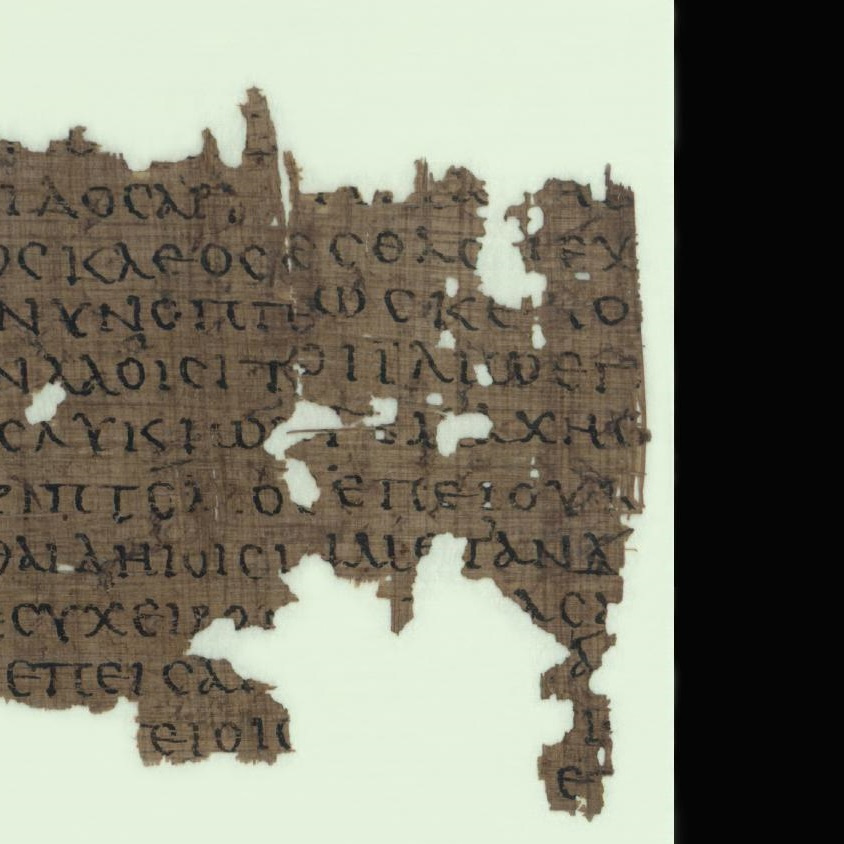
\includegraphics[width=\textwidth]{{raw/G_02317_26742_Pap_crop.jpg}}
        \end{subfigure}
        \hfill
        \begin{subfigure}[b]{0.45\textwidth}
            \centering
            \caption{Example File B}
            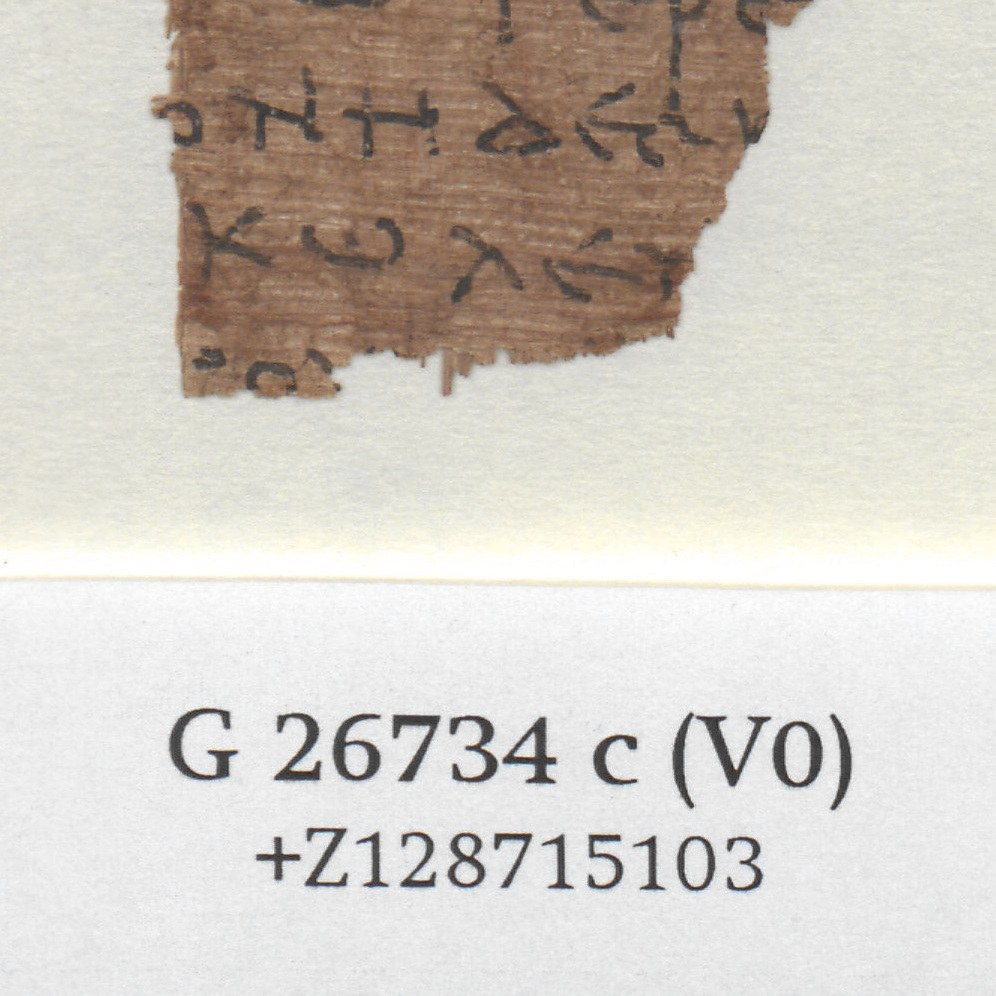
\includegraphics[width=\textwidth]{{raw/G_26734_c_crop.jpg}}
        \end{subfigure}
        \vfill
        \begin{subfigure}[b]{0.45\textwidth}
            \centering
            \caption{Example File C}
            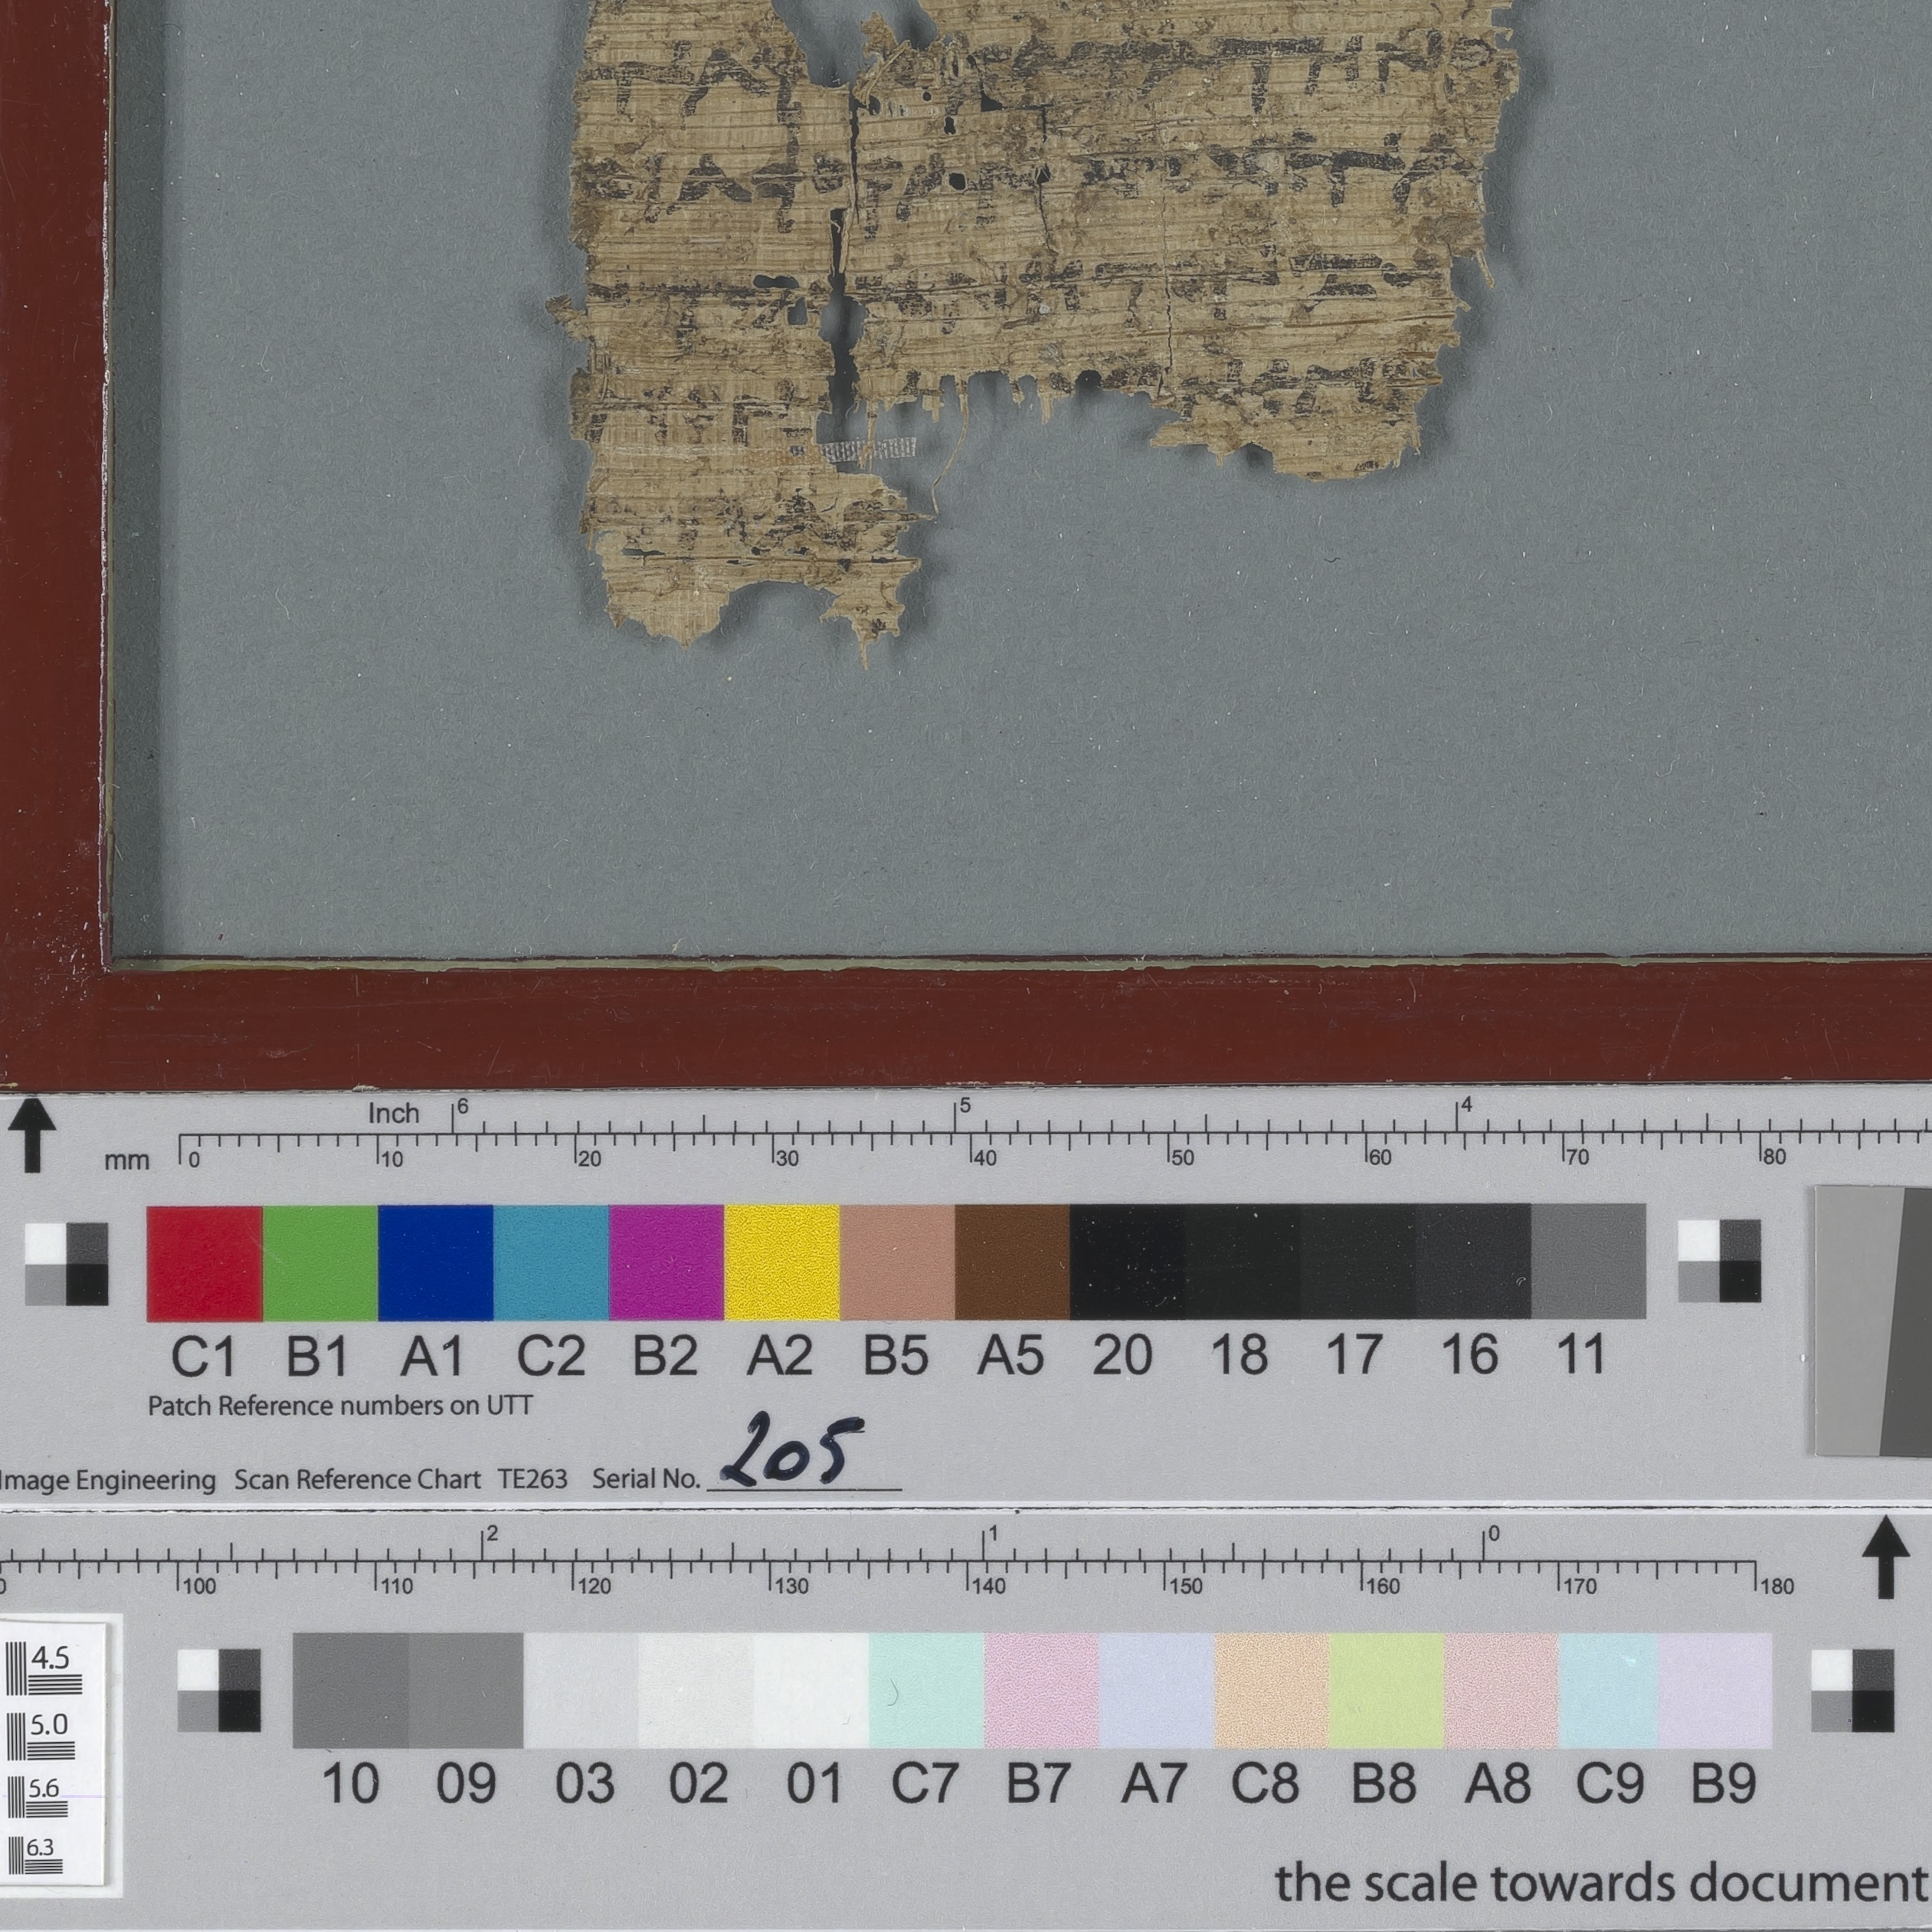
\includegraphics[width=\textwidth]{{raw/P_Hamb_graec_665_crop.jpg}}
        \end{subfigure}
        \hfill
        \begin{subfigure}[b]{0.45\textwidth}
            \centering
            \caption{Example File D}
            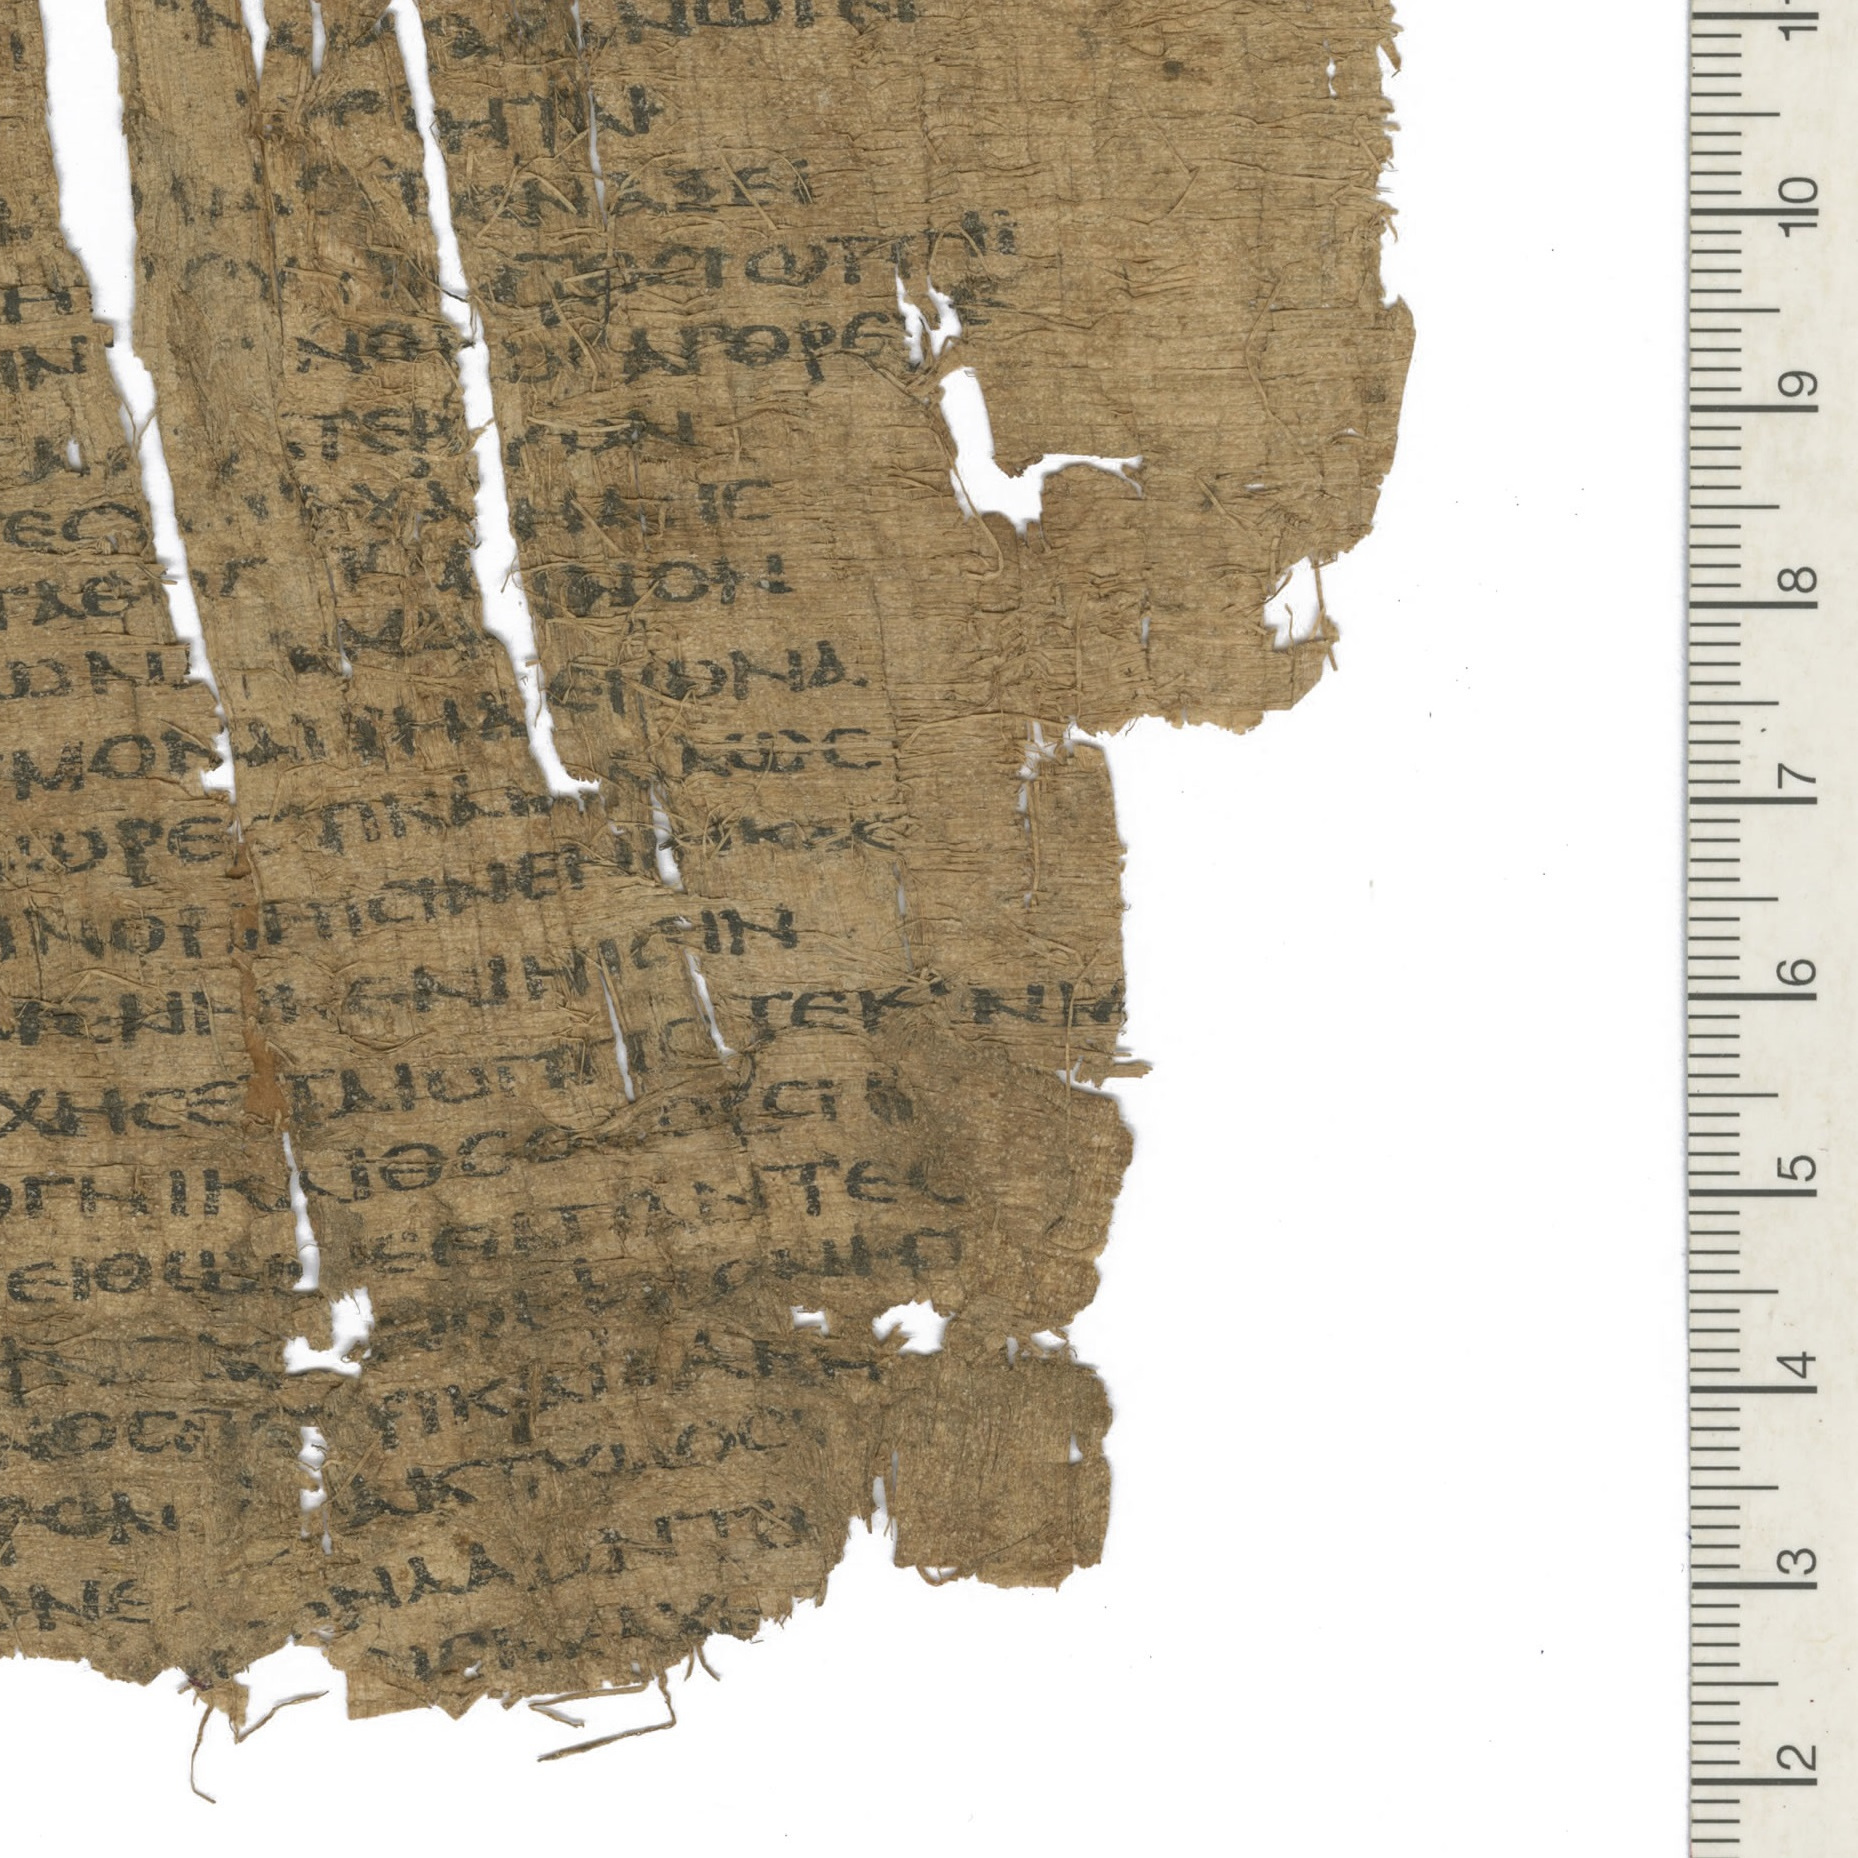
\includegraphics[width=\textwidth]{{raw/PSI_XIV_1377r_crop.jpg}}
        \end{subfigure}
    \end{center}
\end{figure}



\subsection{Clustering}
\todo{NEW, TODO: ADD CONTENT}

\begin{figure}
    \caption{Four Example Binarizations Generated Via Clustering}
    \label{fig:binarizationClustering}
    \begin{center}
        \begin{subfigure}[b]{0.45\textwidth}
            \centering
            \caption{Example File A}
            
\includegraphics[width=\textwidth]{{binarization/clustering/G_02317_26742_Pap_crop.png}}
        \end{subfigure}
        \hfill
        \begin{subfigure}[b]{0.45\textwidth}
            \centering
            \caption{Example File B}
            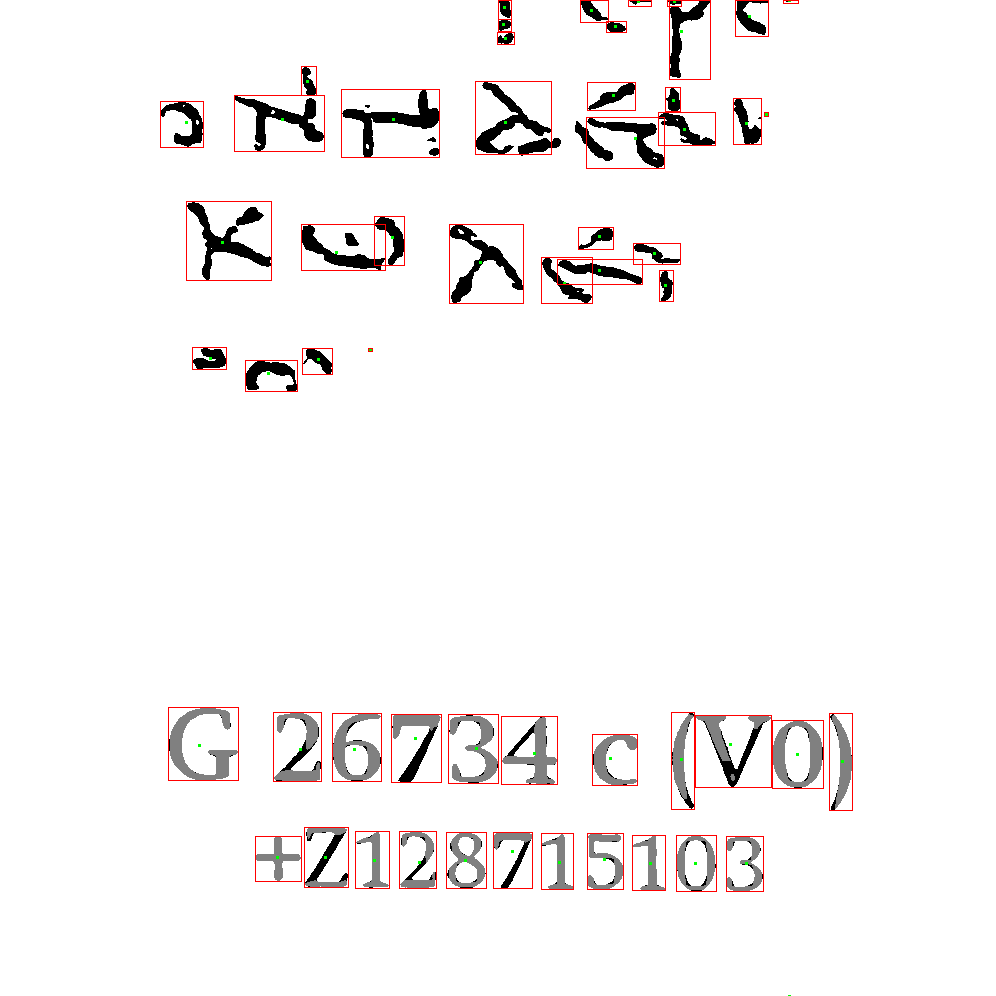
\includegraphics[width=\textwidth]{{binarization/clustering/G_26734_c_crop.png}}
        \end{subfigure}
        \vfill
        \begin{subfigure}[b]{0.45\textwidth}
            \centering
            \caption{Example File C}
            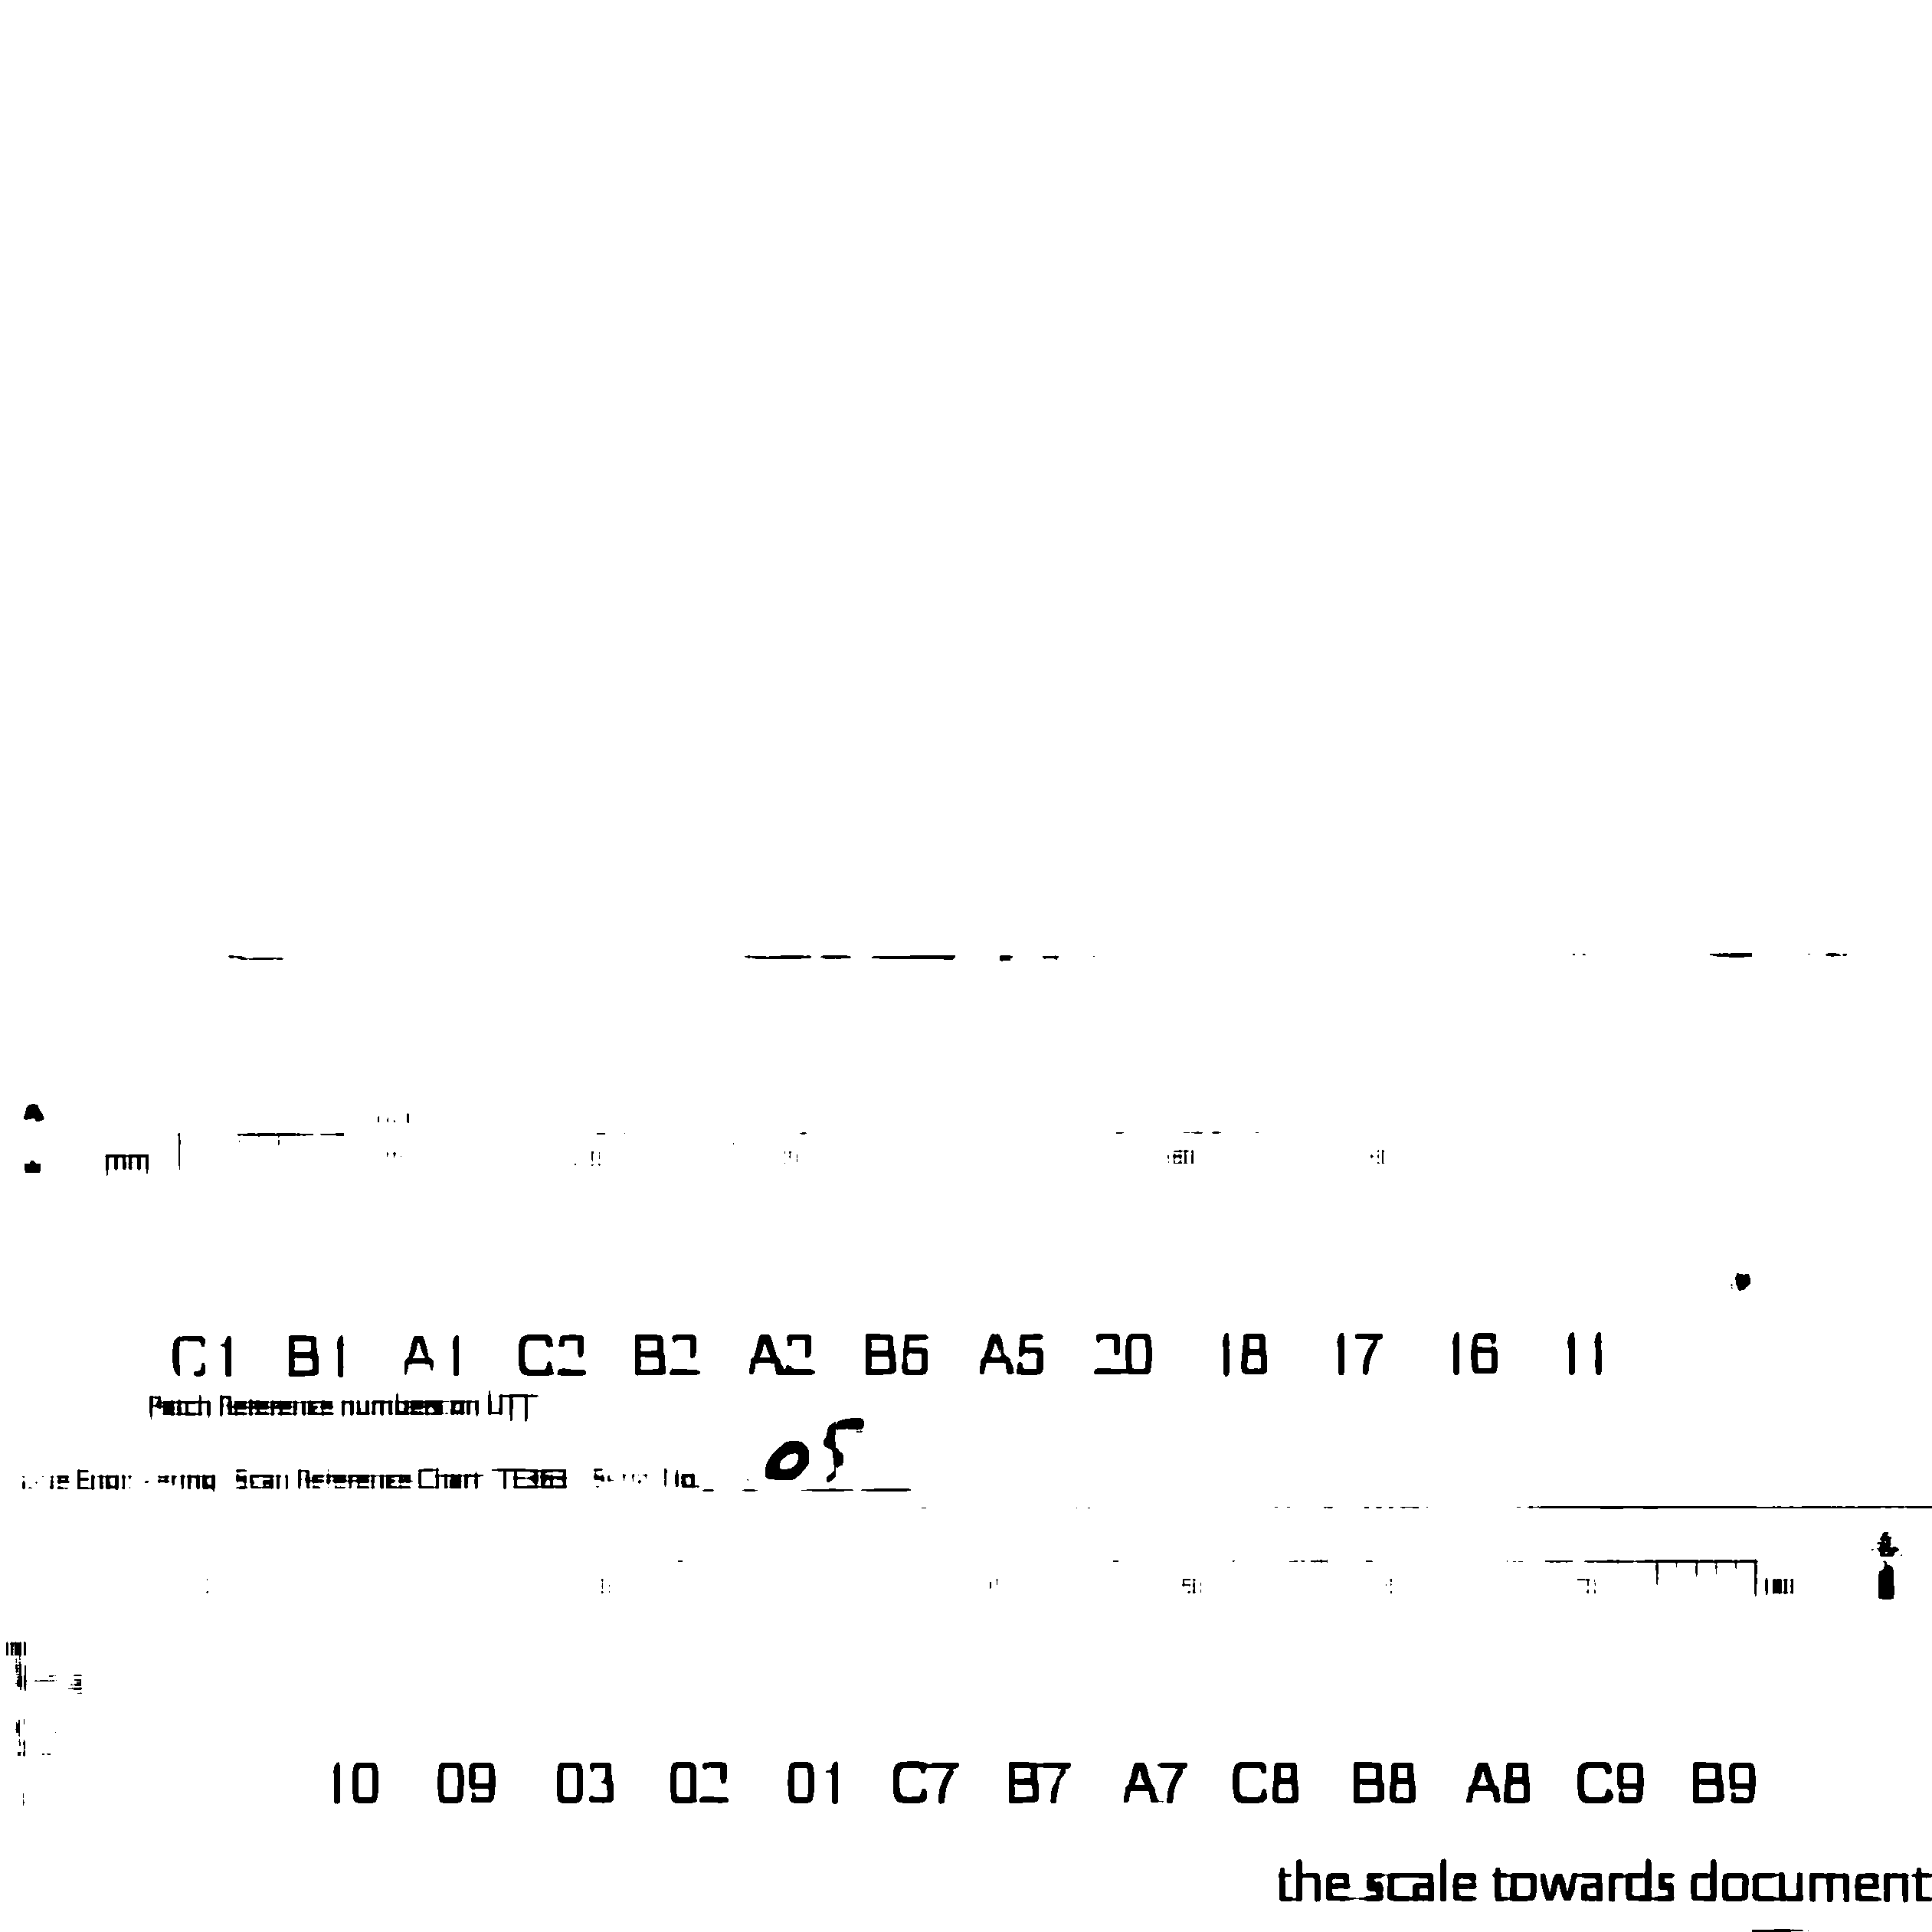
\includegraphics[width=\textwidth]{{binarization/clustering/P_Hamb_graec_665_crop.png}}
        \end{subfigure}
        \hfill
        \begin{subfigure}[b]{0.45\textwidth}
            \centering
            \caption{Example File D}
            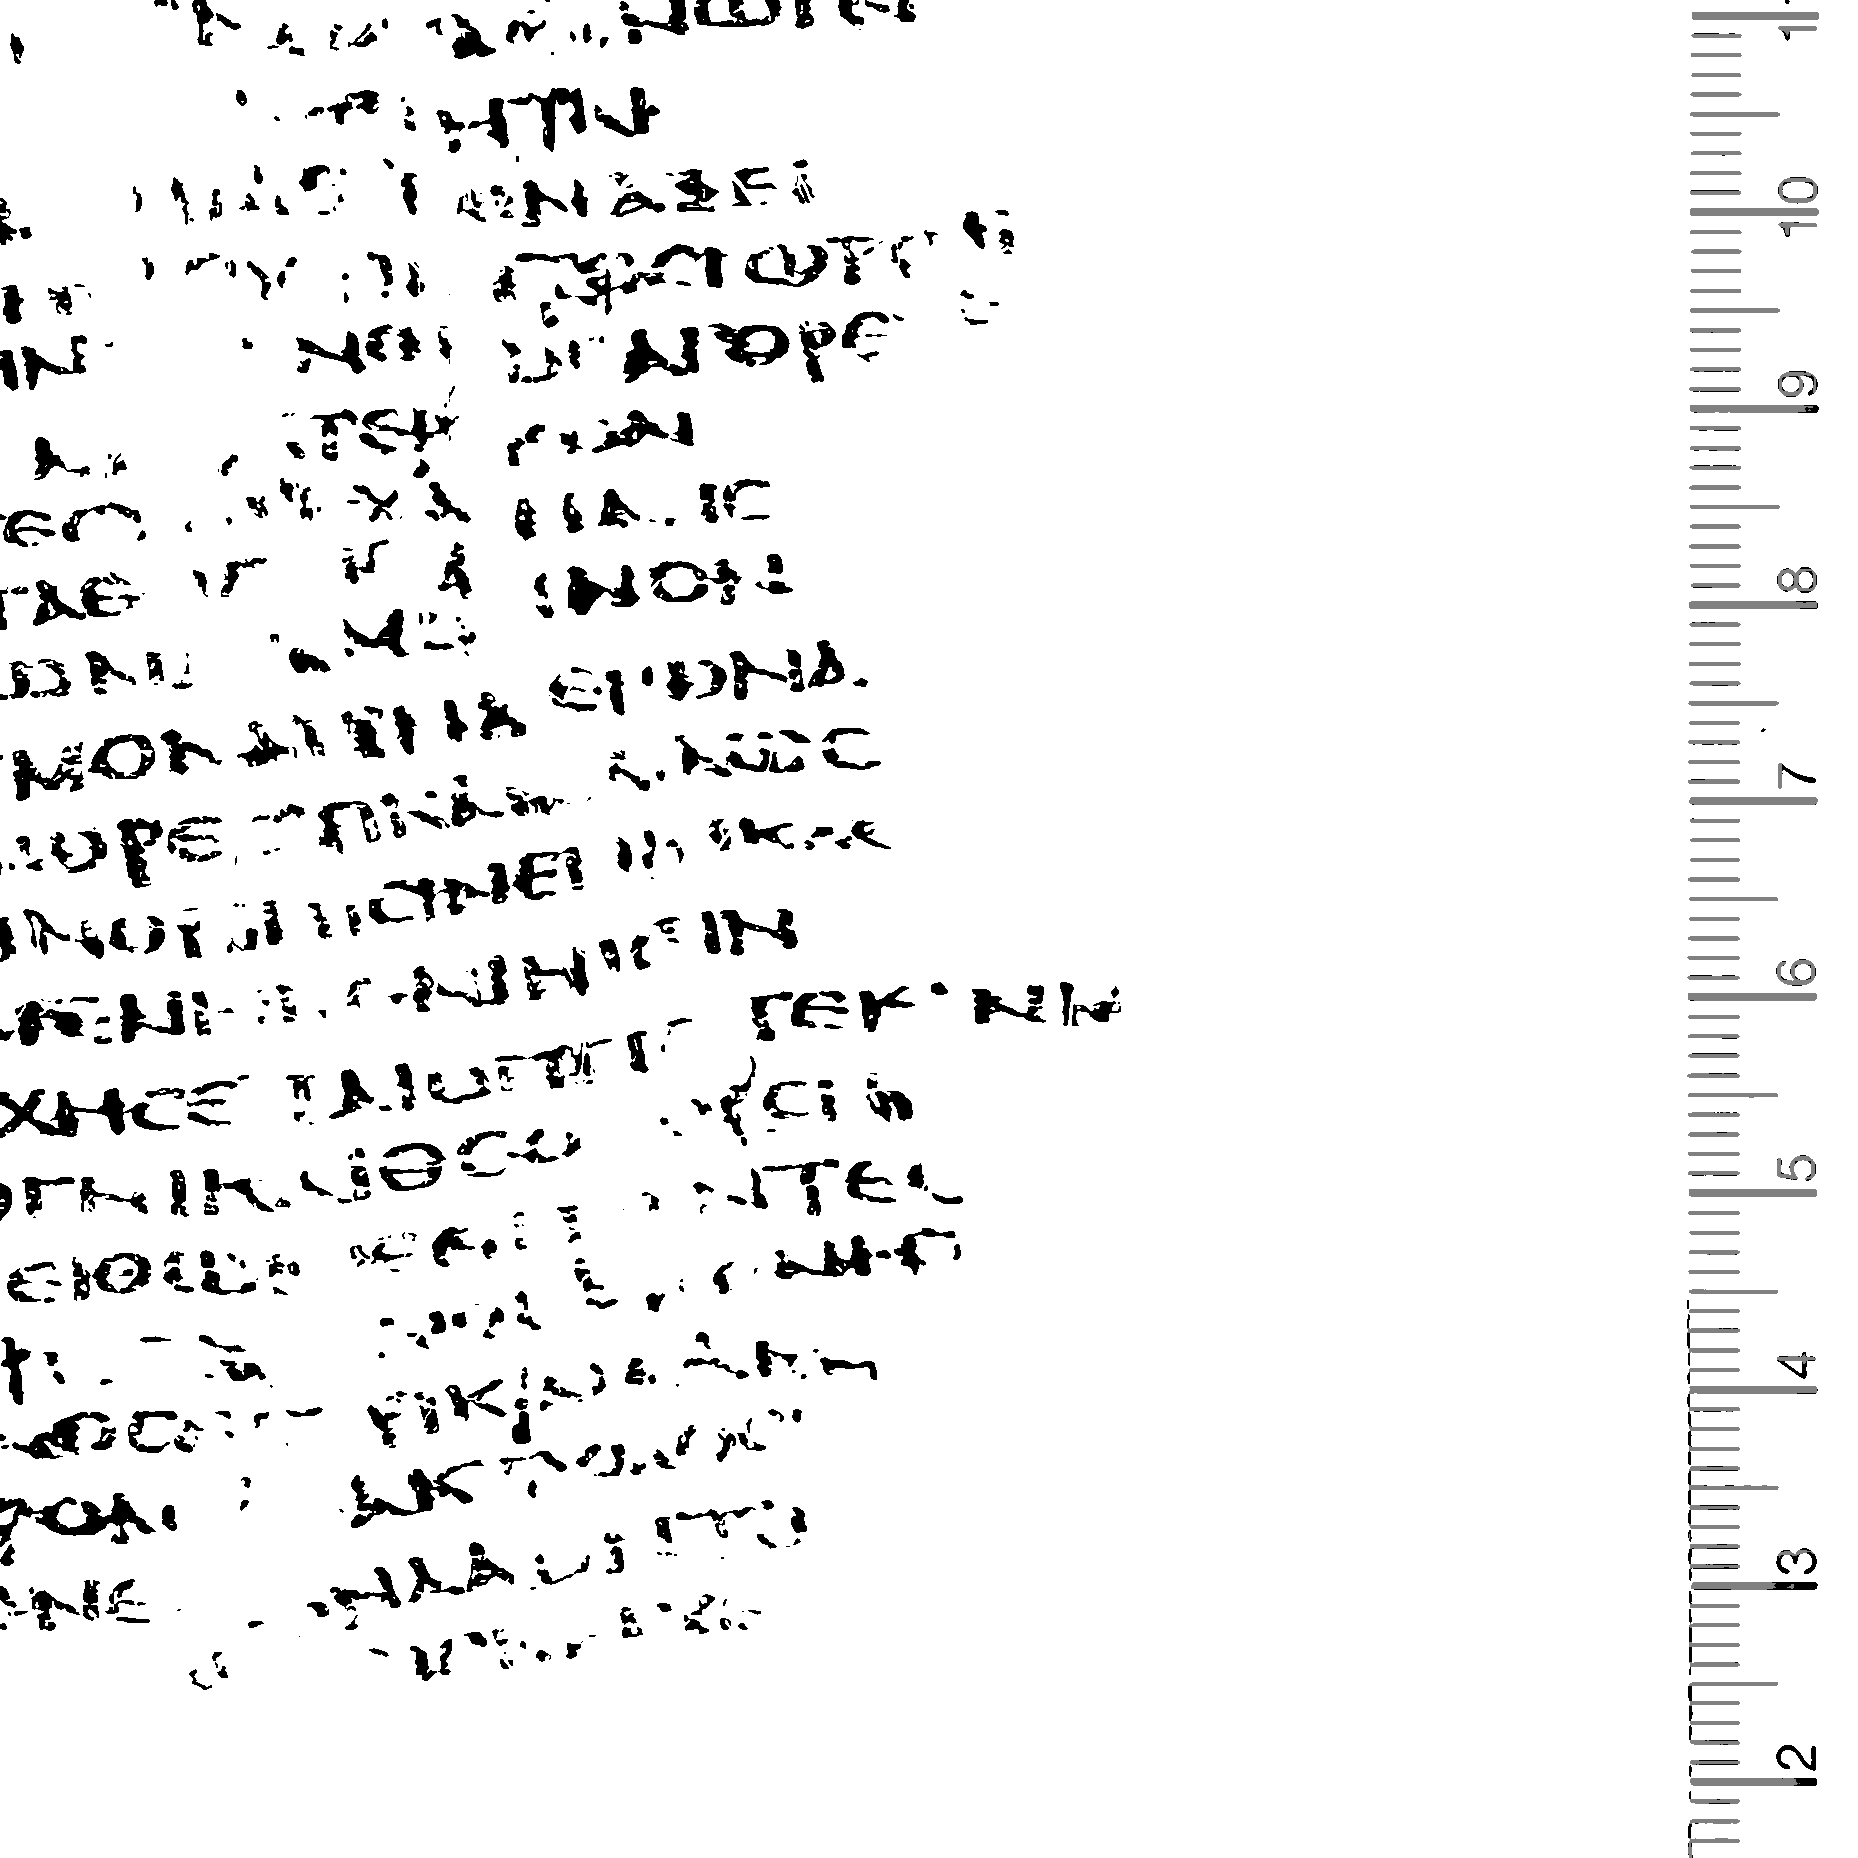
\includegraphics[width=\textwidth]{{binarization/clustering/PSI_XIV_1377r_crop.png}}
        \end{subfigure}
    \end{center}
\end{figure}

\subsection{DP-Linknet}
\todo{TODO: ADD CONTENT}

\subsection{BiNet}
\todo{TODO: ADD CONTENT}


\section{Glyph Bounding}

\subsection{Bounding Boxes}
\todo{TODO: ADD CONTENT}

\subsection{Connected Components}
\todo{TODO: ADD CONTENT}

\subsection{Sliding Window Region Based Convolution Neural Networks}
\todo{TODO: ADD CONTENT}


\section{Line Bounding}

\subsection{Point Of Interest Clustering}
\todo{DOG + POI + adaptive dbscan}

\subsection{Point Of Interest Clustering}
\todo{TODO: ADD CONTENT}

\subsection{Adjacent Glyph Clustering}
\todo{TODO: ADD CONTENT}

\subsection{Overlaping Glyph Clustering}
\todo{TODO: ADD CONTENT}


\section{Classification}

\subsection{Transfer Learning}
\todo{TODO: ADD CONTENT}

\subsection{Convolutional Neural Networks}
\todo{TODO: ADD CONTENT}

\subsection{Stochastic Language Models}
\todo{TODO: ADD CONTENT}

\subsection{Neural Netork Language Models}
\todo{TODO: ADD CONTENT}


\section{Evaluation Metric Analysis}

\subsection{Ground Truth Comparison}
\todo{TODO: ADD CONTENT}

\subsection{Visual Analysis}
\todo{TODO: ADD CONTENT}

\subsection{BLEU Score}
\cite{Callison-Burch}
